\documentclass[lang=cn,zihao=5,twoside,fontset=none]{textbook}
\usepackage{lipsum,zhlipsum}
% ----------------------------- Math Font ------------------------------------- %
% \usepackage{newtxmath}
% \DeclareSymbolFont{CMlargesymbols}{OMX}{cmex}{m}{n}
% \let\sum\relax
% \let\prod\relax
% \DeclareMathSymbol{\sum}{\mathop}{CMlargesymbols}{"50}
% \DeclareMathSymbol{\prod}{\mathop}{CMlargesymbols}{"51}
% %% \infty
% \DeclareSymbolFont{symbolsCM}{OMS}{cmsy}{m}{n}
% \SetSymbolFont{symbolsCM}{bold}{OMS}{cmsy}{b}{n}
% \let\txinfty\infty
% \DeclareMathSymbol{\infty}{\mathord}{symbolsCM}{"31}
\usepackage{amssymb}
\let\heavymath\relax
\let\Bbbk\relax
\usepackage{mtpro2}
\DeclareSymbolFont{CMlargesymbols}{OMX}{cmex}{m}{n}
\let\sum\relax
\let\prod\relax
\DeclareMathSymbol{\sum}{\mathop}{CMlargesymbols}{"50}
\DeclareMathSymbol{\prod}{\mathop}{CMlargesymbols}{"51}
%% \infty
\DeclareSymbolFont{symbolsCM}{OMS}{cmsy}{m}{n}
\SetSymbolFont{symbolsCM}{bold}{OMS}{cmsy}{b}{n}

\DeclareMathSymbol{\infty}{\mathord}{symbolsCM}{"31}

\definecolor{nuanbai}{HTML}{f5f5f5}
\pagecolor{nuanbai}
% ---------------------------------------------------------------------------- %
\overfullrule=5pt
% \showboxdepth=\maxdimen
% \showboxbreadth=\maxdimen
\tracingonline=1
\tracingoutput=1
\usepackage{extarrows}
\addbibresource{ref.bib}
\begin{document}
%----------------------------------------------------------------------------------------
%	标题页信息
%----------------------------------------------------------------------------------------
\title{中文TextBook模板\\A \LaTeX Template for Books in Chinese}
\subtitle{\textit{对一个惊艳的报告样式的复刻}}
\author{Ethan Lu}
\date{\zhtoday}
\publishers{家里蹲出版社}
%----------------------------------------------------------------------------------------

%----------------------------------------------------------------------------------------
%	插入自定义标题页
%----------------------------------------------------------------------------------------
\begin{titlepage} % 创建一个新的页面
    %用来将图片从左下角开始平铺整个封面
        \AddToShipoutPicture*{%
        \AtPageLowerLeft{%
            \adjustbox{width=1.1\paperwidth, height=1.5\paperheight, keepaspectratio}{% 强制图片至纸张尺寸,但可能裁切
                
\includegraphics{images/pexels-photo-3378916.jpeg}
            }
        }
    }
    \begin{flushleft} % 左对齐环境
        \setlength{\leftskip}{1cm} % 左侧缩进
        \makeatletter % 允许访问带有@字符的内部命令
        % \vspace*{4cm} % 标题距离页面顶端的空白
        % {\color{white}\Huge \textbf{\@title} \par} % 使用前文定义的title作为标题
        % \vspace{1cm} % 标题和子标题的间距
        % {\color{white}\Large \@subtitle \par} % 使用前文定义的subtitle作为子标题
        % \vfill % 作者信息前的垂直填充
        % {\color{white}\large \@author \par} % 作者名
        % {\color{white}\large \@publishers \par} % 出版者
        % {\color{white}\large \today\par} % 日期,默认为当天
            \begin{tikzpicture}[overlay,remember picture]
            \begin{pgfonlayer}{bottom}
                \fill[dblue!10,opacity=0.1] (current page.south west) rectangle ++(\paperwidth,2cm);
                \node[inner sep=0pt,text=white,font=\large\sffamily,above] (bottominfo) at ([yshift=.7cm]current page.south) {
                    \@author\hspace{4cm}\@publishers\hspace{4cm}\today
                };
            \end{pgfonlayer}
            \fill[color=black!50,opacity=.2]node[append after command={
                ([yshift=0.5cm]bookinfo.north west) rectangle ([yshift=-0.5cm]bookinfo.south east)},minimum width=\paperwidth,opacity=1,align=left,inner sep=0pt,anchor=west] (bookinfo) at ([shift={(0,4cm)}]current page.west) {\hspace{-7cm}
                    \begin{varwidth}{\linewidth}
                        \setlength\baselineskip{6ex}
                        \textcolor{black!10!white}{\Huge \textbf{\@title}} \\[.6cm]
                        \textcolor{black!10!white}{\Large \@subtitle}
                    \end{varwidth}
                    };
        \end{tikzpicture}
        \makeatother % 将@重置为非字母字符
        \vspace{0cm} % 标题和子标题的间距
        % 结束左对齐环境
    \end{flushleft}
    \ClearShipoutPicture % 清除背景图片
    \end{titlepage}
% --------------------------------- 主要内容写在下面 --------------------------------- %
\pagestyle{Mainpage} % 页面样式
\chapimg{images/pexels-photo-1452701.jpeg}

\begin{titlepage}
    \newgeometry{left=2cm,right=2cm,top=2.5cm,bottom=2.2cm}
    \tableofcontents
    \restoregeometry
\end{titlepage}

% ---------------------------------------------------------------------------- %

\partimg{images/pexels-photo-931018.jpeg}
\part{Intersection Homology}

\chapter{ChatGPT回答}


\section{Intersection Homology and Perverse Sheaves}
\textbf{intersection homology} 比经典的 \textbf{intersection theory} 更适合处理带有奇异点(singularities)的情形。

\subsection{理由}

\begin{enumerate}[label=\arabic*)]
\item \textbf{Poincaré对偶性 (Poincaré Duality)}:
    \textbf{经典同调理论}(包括经典交叉理论)在处理光滑流形(即无奇异点的流形)时,具有良好的对偶性性质,例如 Poincaré对偶性,即在一个紧致无边界的光滑流形上,其同调与上同调之间存在自然的对偶性。然而,当流形有奇异点时,经典同调理论的这些良好性质可能会丢失,Poincaré对偶性在一般奇异空间上不再成立。\textbf{交叉同调 (Intersection Homology)} 是一种修正的同调理论,通过引入“perversity”函数来控制链的支撑在奇异部分的行为,从而在带有奇异点的空间上恢复了 Poincaré对偶性。因此,intersection homology 是更为适合奇异空间的一个理论工具。
	\item \textbf{奇异点的处理}:
   在经典的交叉理论中,处理奇异点的交叉通常是困难且不精确的,因为交叉产品在奇异点上可能产生不可预期的结果,甚至可能失去其几何意义。
   交叉同调通过将同调链的选取限定在具有一定“良好行为”的链(即满足 perversity 条件的链)上,避免了许多在奇异点附近的病态行为。这使得交叉同调能够更精确地捕捉奇异空间中的几何和拓扑信息。
   \item \textbf{交叉同调的几何解释}:
   交叉同调理论\sidenote{交叉同调(Intersection Homology)相较于经典交叉理论,提供了一种更为强大且适用于带有奇异点的空间的理论工具。它通过对链的支撑条件的限制,在处理奇异点时避免了病态行为,保持了关键的几何和拓扑性质,如 Poincaré对偶性。因此,intersection homology 被广泛认为是在处理奇异空间时比经典交叉理论更为适合和普遍的方法。}为奇异空间上的交叉理论提供了一个更深层次的几何解释。它不仅仅是一个计算工具,还包含了对奇异点的结构性理解。例如,交叉同调的构造可以与 perverse sheaves 联系起来,通过这些 sheaves 的超同调来理解空间的交叉同调。
   \item \textbf{应用与普适性}:
   交叉同调在代数几何、拓扑学和表示论中都有广泛的应用,尤其是在处理具有奇异性的代数簇时。它提供了一种统一的方法来研究这些空间,弥补了经典交叉理论在奇异点处理上的不足。
   在 Decomposition Theorem(分解定理)、Riemann-Hilbert 对应以及表示论的几何化等现代数学的重要领域中,交叉同调及其关联的 perverse sheaves 都扮演着至关重要的角色。
\end{enumerate}

\section{Poincar\'e Duality}

\begin{theorem}[Poincar\'e Duality]\label{thm:poincare-duality}
	Let $X$ be a closed, connected, oriented topological $n$-manifold with fundamental class $[X]$. Then capping with $[X]$ gives an isomorphism
	\[H^i(X,\bZ)\xlongrightarrow[]{\cong} H_{n-i}(X,\bZ)\]
	for all integers $i$.
\end{theorem}

在代数拓扑中,“\textbf{cap product}\sidenote{这里的 cap product 还需要去代数拓扑中深入学习!}” 是一种将上同调与同调结合起来的运算,这与“cup product” 是相对的。你已经熟悉了 cup product,这是一种将两个上同调群的元素结合起来的二元运算,而 cap product 则是涉及上同调群与同调群的一种运算。

具体来说,cap product 是一种运算,它将一个上同调类(来自 $H^i(X)$)和一个同调类(来自 $H_n(X)$)结合起来,得到一个较低维度的同调类(来自 $H_{n-i}(X)$)。

在你提供的图片中,定义 cap product 是为了说明 Poincaré 对偶性。对于一个 $n$ 维流形 $X$,cap product 使得我们可以将一个上同调类与一个基本类(fundamental class)结合起来,并得到一个特定维度的同调类。

公式中的 cap product 形式化地写作:
$$
\color{purple}
C^i(X) \times C_n(X) \rightarrow C_{n-i}(X)
$$
其中 $C^i(X)$ 是 $X$ 上 $i$ 维(单纯/奇异)链的上同调群,而 $C_n(X)$ 是 $X$ 上 $n$ 维链的同调群。这个运算定义为:
$$
a(b \cap \sigma) = (a \cup b)(\sigma),
$$
这个等式左边是关于 cap product 的描述,其中 \( a \) 是一个来自 \( C^{n-i}(X) \) 的上同调类,\( b \) 是一个来自 \( C^i(X) \) 的上同调类,而 \( \sigma \) 是来自 \( C_n(X) \) 的同调类。

右边的 \( (a \cup b)(\sigma) \) 表示一种“作用”,具体来说是 \( a \) 和 \( b \) 在链 \( \sigma \) 上的作用。这里的 \( \cup \) 代表的是两者的结合(组合)产生一个新的上同调类,而这个新类通过作用在链 \( \sigma \) 上,得到一个具体的值。这并不是 cup product,而是将两个上同调类合并,并将其作用在一个具体的链上。

因此,正确理解是:在这个上下文中,\( \cup \) 只是表示将上同调类 \( a \) 和 \( b \) 结合,而不是典型的 cup product 运算,它实际上是一个关于映射和链的自然作用。

再一次总结:左边的 \( \cap \) 是 cap product,它将上同调类和同调类结合,产生一个新的同调类;右边的 \( \cup \) 是表示将上同调类 \( a \) 和 \( b \) 作用到链 \( \sigma \) 上的结合,并得出一个值。
\begin{remark}
	一个同调群里面的元素是什么?假设$X$是一个$n$流形。

\textbf{答:}在同调群中,元素通常是\textbf{同调类},这些同调类由链群中的“链”生成,通过边界算子的作用归约到等价类中。让我们更系统地分析这个问题,假设 $X$ 是一个 $n$- 维流形,则
\paragraph*{1. 链群 ($C_k(X)$)}
首先,同调是基于链复形构建的。在同调论中,对于一个拓扑空间 $X$(如一个 $n$- 维流形),我们可以构建链群 $C_k(X)$,它由 $k$- 维\textbf{单形}(或者更一般地是链)生成。这些单形是连续地从标准 $k$- 维单形 $\Delta^k$ 到 $X$ 的映射。
\begin{enumerate}
	\item \textbf{生成元}: $k$- 维单形(可以看作一个几何对象,如线段、三角形等)。
	\item\textbf{线性组合}:链群是由这些单形的自由阿贝尔群生成的。因此,链可以看作这些单形的线性组合。
\end{enumerate}
例如,若 $X$ 是一个二维流形,链群 $C_2(X)$ 包含三角形之类的 2- 单形,$C_1(X)$ 包含边(线段),而 $C_0(X)$ 则包含顶点。

\paragraph*{2. 边界算子 ($\partial_k$)}
对于每一个链群 $C_k(X)$,都有一个边界算子 $\partial_k$,它将 $k$- 维链映射到其边界的 $(k-1)$- 维链。例如,一个三角形的边界是它的三条边(线段),而一条边的边界是它的两个端点。

边界算子满足 $\partial_k \circ \partial_{k+1} = 0$,即“边界的边界为零”。这就是构成同调论的链复形的基础。

\paragraph*{3. 同调群 ($H_k(X)$)}
同调群定义为边界链和循环链的商群。我们通过边界算子在链群中引入了两个重要的子群:
\begin{enumerate}
	\item \textbf{循环群} $Z_k(X)$ (cycles):这是满足 $\partial_k \sigma = 0$ 的所有 $k$- 维链的集合。它们没有边界,可以认为是“闭合的”链。
	\item\textbf{边界群} $B_k(X)$(boundaries):这是可以写作 $\sigma = \partial_{k+1} \tau$ 的所有 $k$- 维链的集合。这些链是某个更高维链的边界。
\end{enumerate}
那么,$k$- 维同调群 $H_k(X)$ 定义为:
$$
\color{purple}
H_k(X) = Z_k(X) / B_k(X)
$$
即,所有的循环链的集合,模掉那些实际上是边界的链。

\paragraph*{4. 同调群中的元素}
\textbf{同调类}:同调群 $H_k(X)$ 的元素被称为 $k$- 同调类,它代表了一类等价的 $k$- 维循环链,等价类是模去那些可以被写作边界的链(即模掉边界群)。因此,同调群中的元素可以理解为某个不属于边界的闭链(比如流形中的某个闭合的几何对象)。

例如,在一个二维流形上,$H_2(X)$ 中的元素可能代表流形上的整个闭合区域,$H_1(X)$ 中的元素可能代表闭合的环路,而 $H_0(X)$ 中的元素则对应于不同的连通分量。

\paragraph*{5. 基本类 (Fundamental Class)}
如果 $X$ 是一个 $n$- 维定向流形,它有一个特别重要的同调类,称为\textbf{基本类}(fundamental class),记为 $[X]$。这是 $H_n(X)$ 中的一个生成元,代表整个流形本身作为一个 $n$- 维链。Poincaré 对偶性正是依赖于基本类的存在,表明 $n$- 维同调和 $0$- 维上同调之间的关系。

总结:对于一个 $n$- 维流形 $X$,同调群中的元素是同调类,通常代表的是流形中的几何对象(闭链):
\begin{itemize}
	\item $H_0(X)$:连通分量的数目;
	\item $H_1(X)$:闭合的环路;
	\item $H_2(X)$:闭合的曲面或区域;
	\item $H_n(X)$:通常是基本类 $[X]$,代表整个流形本身。
\end{itemize}
同调类将几何对象的形状和拓扑性质联系起来,并通过 Poincaré 对偶性与上同调群之间建立深刻的联系。
\end{remark}

请问基于上面的图片,1.如何推导得到第一个非退化的配对?2. 如何推导得到第二个式子的Betti数关于互补同调次数下相等?如何理解?
\begin{figure}[htbp]
	\centering
	\sidecaption{两个重要推论的理解\label{fig:two-vital-corollaries}}{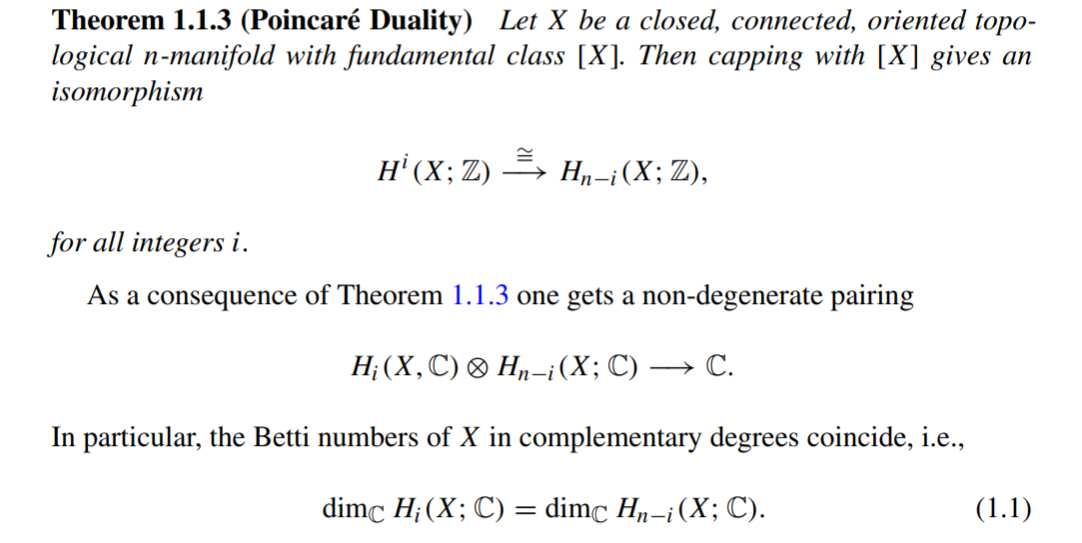
\includegraphics[width=.7\textwidth]{images/PixPin_2024-09-05_09-23-13.png}}
\end{figure}

\begin{solution}
	1. \textbf{如何推导第一个非退化的配对?}

第一个非退化的配对源自\textbf{庞加莱对偶定理}(Poincaré Duality Theorem),该定理对紧闭的定向流形 $X$ 给出了拓扑性质之间的深刻联系。通过该定理,我们能够在不同的同调次数之间建立一种自然的配对关系。

庞加莱对偶定理表明,对于一个 $n$- 维的紧闭定向流形 $X$,存在一个同构:
$$
H^i(X; \mathbb{Z}) \cong H_{n-i}(X; \mathbb{Z}),
$$
这个同构是通过与基本类 $[X]$ 的\textbf{帽积}(capping product)定义的。设 $\alpha \in H^i(X; \mathbb{Z})$,则将 $\alpha$ 与 $[X]$ 取帽积:
$$
\alpha \cap [X] \in H_{n-i}(X; \mathbb{Z}),
$$
该映射实际上是一个同构。

基于此同构,我们可以构造一个非退化的配对:
$$
H_i(X; \mathbb{C}) \otimes H_{n-i}(X; \mathbb{C}) \rightarrow \mathbb{C},
$$
这意味着两个同调群之间存在一个自然的双线性配对关系,且该配对是非退化的(即没有非零的元素被映射到零)。这来自于拓扑中的\textbf{对偶性},将 $H_i(X; \mathbb{C})$ 中的元素和 $H_{n-i}(X; \mathbb{C})$ 中的元素成对映射到 $\mathbb{C}$ 中。

\paragraph*{如何理解?}
这一配对的几何解释可以理解为:一个 $i$- 维同调类可以与一个 $(n-i)$- 维同调类进行相交,结果是一个数值(例如,两个闭链相交的点数)。这种配对反映了流形内部不同维度之间的相互关系,从而提供了深刻的几何和拓扑结构上的联系。

2. \textbf{如何推导 Betti 数在互补同调次数下相等?}

Betti 数是同调群的维数,具体来说:$b_i = \dim H_i(X; \mathbb{C})$ 表示第 $i$ 个同调群的复数维数。

庞加莱对偶定理告诉我们 $H^i(X; \mathbb{Z}) \cong H_{n-i}(X; \mathbb{Z})$,因此通过复数系数的推广,这意味着在复数系下,同调群 $H_i(X; \mathbb{C})$ 和 $H_{n-i}(X; \mathbb{C})$ 的维数必须相等。

因此,Betti 数满足以下关系:
$$
\dim_{\mathbb{C}} H_i(X; \mathbb{C}) = \dim_{\mathbb{C}} H_{n-i}(X; \mathbb{C}),
$$
即在互补同调次数 $i$ 和 $n-i$ 下,Betti 数相等。

\paragraph*{如何理解?}
这一等式的几何意义反映了流形在不同维度上具有对称性。由于庞加莱对偶定理中的配对关系,我们可以认为流形的高维拓扑特性(例如 $H_i$)与其低维特性(例如 $H_{n-i}$)之间存在一种对偶关系。这使得流形的同调群维度在互补维度上保持一致,表明了流形在几何和拓扑结构上的对称性。


\end{solution}

\begin{problem}[例1理解]\label{thm:}
	如何理解?
\end{problem}

		\begin{figure}[htbp]
			\centering
		\sidecaption{例1理解\label{fig:example1}}{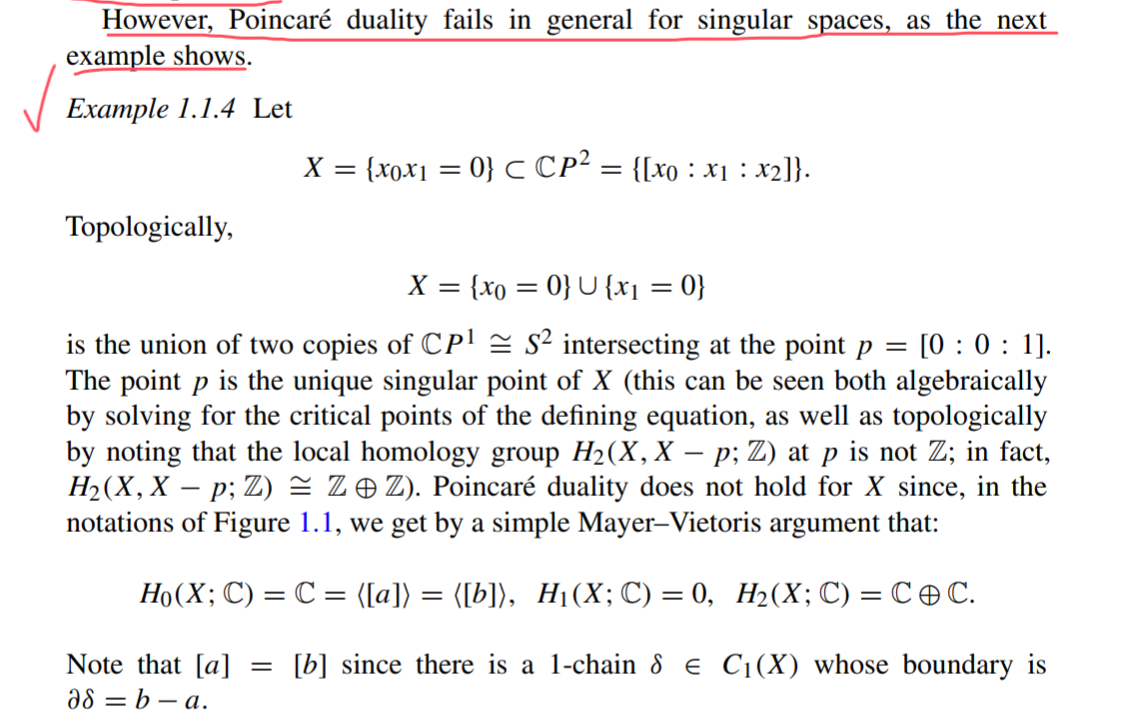
\includegraphics[width=.7\textwidth]{images/PixPin_2024-09-05_10-38-34.png}}
	\end{figure}



\begin{solution}
	这个例子(例 1.1.4)展示了庞加莱对偶定理在奇异空间上的失败。

\subsubsection{空间 $X$ 及其奇异点:}

1. $X = \{ x_0 x_1 = 0 \} \subset \mathbb{C}P^2$ 是复射影平面中的一个曲面,由两条坐标轴 $x_0 = 0$ 和 $x_1 = 0$ 组成。拓扑上,这个空间是两个 $\mathbb{C}P^1$(拓扑上同胚于 $S^2$)的并集。

2. 这两个 $\mathbb{C}P^1$ 在点 $p = [0 : 0 : 1]$ 相交,该点是 $X$ 的唯一奇异点。

\subsubsection{奇异点的局部同调性质:}

在奇异点 $p$,局部同调群 $H_2(X, X - p; \mathbb{Z})$ 不再是 $\mathbb{Z}$,而是 $\mathbb{Z} \oplus \mathbb{Z}$。这是因为 $X$ 在 $p$ 处的结构与普通平滑流形不同。奇异点使得局部同调群的性质发生了改变,从而影响了庞加莱对偶定理的成立。

\subsubsection{为什么庞加莱对偶定理失败:}

在这个奇异空间 $X$ 上,庞加莱对偶定理不再成立。具体来说,使用\textbf{Mayer-Vietoris 序列}可以计算出 $X$ 的同调群:
- $H_0(X; \mathbb{C}) = \mathbb{C}$,表明 $X$ 是连通的。
- $H_1(X; \mathbb{C}) = 0$,表明 $X$ 没有非平凡的 1 维环。
- $H_2(X; \mathbb{C}) = \mathbb{C} \oplus \mathbb{C}$,表明 $X$ 有两个独立的 2 维同调类,反映了两个 $S^2$ 的并集。

在普通的平滑流形上,庞加莱对偶定理会给出 $H_0$ 与 $H_2$ 之间的对偶关系(它们的维数相同),以及 $H_1$ 的对偶性(即 $H_1$ 与 $H_1$ 的自对偶)。然而,这里 $H_2(X; \mathbb{C}) = \mathbb{C} \oplus \mathbb{C}$ 显示了该空间的局部奇异性破坏了通常的对偶关系。

\subsubsection{结论:}

由于空间 $X$ 有奇异点,庞加莱对偶定理不再适用。这展示了在奇异空间中,流形的局部拓扑结构对全局同调特性的影响,特别是在同调群的计算中出现了不同寻常的情况,使得对偶关系无法成立。


\end{solution}



复射影空间 $\mathbb{C}P^2$ 是一个复杂的几何结构,但我们可以通过一定的直观手段理解其结构,并试着描述它的图像。

\subsubsection{定义}
$\mathbb{C}P^2$ 是由所有非零复数向量 $(z_0, z_1, z_2) \in \mathbb{C}^3$ 的等价类构成的空间,其中两个向量是等价的当且仅当它们通过一个非零复数相乘得到,即:
\[
(z_0, z_1, z_2) \sim (\lambda z_0, \lambda z_1, \lambda z_2) \quad \text{对于} \ \lambda \in \mathbb{C}^*.
\]
每个等价类表示的是复数平面中通过原点的一条直线。

\subsubsection{可视化的几何形象}
虽然 $\mathbb{C}P^2$ 是一个四维复流形(实维度为 4),我们可以通过一些简单的情况来获得一个有限的直观理解:

1. \textbf{类比于 $\mathbb{C}P^1$}:复射影直线 $\mathbb{C}P^1$ 可以看作是二维球面 $S^2$,因为 $\mathbb{C}P^1$ 是由复平面中通过原点的所有直线组成。类似地,$\mathbb{C}P^2$ 是由三维复空间 $\mathbb{C}^3$ 中的直线组成,但由于它的维度更高,无法直接画出。

2. \textbf{嵌入三维的形象}:$\mathbb{C}P^2$ 可以嵌入到更高维的实空间中。通过某些低维投影的方式,可以想象 $\mathbb{C}P^2$ 是某种“曲面”的延展,这种曲面类似于 $\mathbb{C}P^1$ 在复射影空间中的延伸。其局部片段看起来像是复杂的、相互联系的“球面”或“曲面”,但其结构在全局上更加复杂。

3. \textbf{Fubini-Study 度量的理解}:$\mathbb{C}P^2$ 配备了 Fubini-Study 度量,这使它具有对称性和复杂的几何结构。这种度量定义了 $\mathbb{C}P^2$ 的局部几何性质,使得其形象更像是一个弯曲的、多维的球面,但我们只能通过投影来部分理解它。

\subsubsection{常用的几何表示}
虽然我们无法真正画出 $\mathbb{C}P^2$,但可以通过简单的示意图来表示其分支结构。例如,可以通过以下方法来理解它:
- 将 $\mathbb{C}P^2$ 看作是两个复杂坐标平面的并集,它们在某些奇异点相交。
- 类似于二维平面中的射影线,我们可以在三维空间中可视化射影平面的投影,这就像是从一个高维球面上取投影一样。

\subsubsection{图像类比}
可以将 $\mathbb{C}P^2$ 想象为一种“高维的球面”或“曲面”的扩展,它的图像是无法直接可视化的。但可以通过简单的 $\mathbb{C}P^1$ 来得到一定的类比,比如:
- $\mathbb{C}P^1$ 是 $S^2$。
- $\mathbb{C}P^2$ 是更高维的推广,类似于 $S^4$ 的曲面。

虽然这种类比不完全精确,但它可以帮助我们理解 $\mathbb{C}P^2$ 的几何复杂性。

\chapter{复几何的研究热点及未来可能的热门问题探讨}

\section{问题罗列}

在复几何领域,仍有许多未解决的问题和研究方向,以下是一些当前可以研究的热点问题和挑战:

\paragraph*{1. \textbf{霍奇猜想(Hodge Conjecture)}}
   霍奇猜想是复几何和代数几何中最重要的未解难题之一。它涉及在复代数簇上的代数闭链是否可以表示为复代数闭链的线性组合。虽然霍奇猜想在某些特殊情况下已被证明,但在一般情况下仍未解决。

\paragraph*{2. \textbf{极小模型计划(Minimal Model Program, MMP)}}
   极小模型计划是代数几何的核心项目之一,其目的是通过对代数簇进行某些特殊变换,来研究其结构。虽然在某些维数的情况下,这一计划取得了进展,但在高维情形下,仍有很多问题需要进一步探索,特别是涉及复几何结构的情形。

\paragraph*{3. \textbf{凯勒 - 爱因斯坦度量(Kähler-Einstein Metrics)}}
   研究凯勒流形上的凯勒 - 爱因斯坦度量是复几何的核心问题之一,特别是在非正曲率的情形下。这一问题与微分几何和复几何之间有着深刻的联系。虽然在某些情形下凯勒 - 爱因斯坦度量已经被构造出来,但在更一般的情形下,寻找这些度量仍然是一个具有挑战性的问题。

\paragraph*{4. \textbf{镜像对称性(Mirror Symmetry)}}
   镜像对称性是弦理论中提出的一种数学猜想,它联系了两种不同类型的卡拉比 - 丘流形(Calabi-Yau manifolds)。这不仅是物理学中的重要问题,同时也是复几何的前沿研究领域。镜像对称性的完整数学证明和进一步推广仍然是当前研究的重点之一。

\paragraph*{5. \textbf{复流形的分类}}
   虽然某些低维复流形已经被分类清楚,但高维复流形的分类问题仍然非常复杂。研究如何在更高维度上对复流形进行分类,以及理解其几何和拓扑性质,仍然是一个开放的研究领域。

\paragraph*{6. \textbf{特殊拉格朗日子流形(Special Lagrangian Submanifolds)}}
   特殊拉格朗日子流形在镜像对称性理论中起着关键作用。如何构造和研究这些子流形,特别是在卡拉比 - 丘流形中的情形,仍然是一个具有挑战性且富有前景的研究课题。

\paragraph*{7. \textbf{模空间(Moduli Spaces)}}
   研究复几何中的模空间,特别是某些几何对象的模空间(如向量丛、曲线等)仍然是一个活跃的研究领域。模空间的几何结构,尤其是其奇点和紧化问题,仍然有许多未解的难题。

\paragraph*{8. \textbf{辛几何与复几何的联系}}
   辛几何与复几何之间有许多深刻的联系,特别是通过镜像对称性和 Floer 同调理论。研究这些几何理论之间的相互作用和新应用,仍然是一个活跃的研究方向。

这些问题不仅推动了复几何的发展,也与其他数学领域如代数几何、微分几何、辛几何等紧密相连。如果你对这些领域感兴趣,深入研究其中一个问题将是一个很好的起点。

\section{Perverse Sheaves and Intersection Homology}

\textbf{拓扑分层空间}(topologically stratified space)是一个在拓扑学和几何学中经常使用的概念,通常出现在代数几何、微分几何、奇点理论等领域。理解拓扑分层空间的关键在于如何将一个复杂的几何或拓扑空间分解成若干“分层”部分,每一层都具有较为简单的几何结构。

\subsubsection{1. \textbf{定义大致描述}:}
一个\textbf{拓扑分层空间} $X$ 是一个拓扑空间,它被分解为一系列分层(strata),这些分层彼此之间是分离的。每一个分层是一个光滑的流形,而不同分层之间通过特定的方式相互连接。形式上,它通常被定义为:
\begin{itemize}
    \item 一个拓扑空间 $X$ 被分为若干\textbf{分层} $X_i$,即 $X = \bigcup X_i$,
    \item 这些分层按次序满足 $X_i \subseteq \overline{X_j}$ ($X_j$ 的闭包) 当且仅当 $i < j$。换句话说,较低维的分层在较高维的分层的边界上。
\end{itemize}

\subsubsection{2. \textbf{具体解释}:}
 \textbf{简单分层的示例}:一个典型的例子是将复杂的空间分成多个维度递减的部分。举个例子:
 \begin{itemize}
    \item 一个二维圆盘的中心可以看作是一个“零维”分层。
    \item 去掉圆盘中心后剩下的内部区域是一个“二维”的分层。
    \item 因此,我们可以将这个圆盘分成两个分层:中心点和圆盘的其余部分(不包括中心点)。
 \end{itemize}

这是一种非常简单的分层结构,因为我们将圆盘分成不同的维度:零维和二维。

 \textbf{更复杂的例子}:一个三维圆锥(锥面)也可以是一个拓扑分层空间。锥尖是一个零维分层,而锥面去掉锥尖部分是一个二维分层。尽管它是一个三维空间,但它的分层却可以通过分解为不同维度的部分来理解。

\subsubsection{3. \textbf{典型性质}:}
拓扑分层空间的一些关键性质包括:
\begin{itemize}
\item 每个分层都是一个\textbf{流形},即它在局部具有光滑的结构。比如二维的分层看起来像平面,三维的分层看起来像欧几里得空间。
\item 分层之间的连接有一定的规律性,特别是高维分层的边界常常包含低维分层。
\end{itemize}

\subsubsection{4. \textbf{常见的应用}:}
\textbf{代数几何}中的\textbf{奇点理论}:许多复杂空间中的奇点可以通过分层空间来描述。例如,一个代数簇的奇点可以视作高维空间的低维分层;\textbf{微分拓扑学}:在研究特征类或者流形奇点时,拓扑分层空间可以帮助分析几何结构的局部性质。

\subsubsection{5. \textbf{总结}:}
拓扑分层空间本质上是一个复杂拓扑空间的分解,它将这个空间分为多个简单的分层,每个分层的拓扑结构相对容易理解。通过这样的分解,数学家们可以更好地分析复杂空间的几何性质及其奇异行为。


\subsection{Link of a point}

\textbf{The link of a point} 在几何拓扑学中是一个用于描述拓扑空间中某点附近局部结构的概念。它特别常用在分析奇点或分层空间中的奇异点时,可以帮助理解在某点附近的几何形态。链接为我们提供了一种方法来考察一个点周围的“切向”或“环绕”结构,而不涉及那个点本身。

\subsubsection{1. \textbf{定义}:}
给定一个拓扑空间 $X$ 和空间中的某个点 $p$,\textbf{link of a point},记作 $\text{Link}(p)$,可以大致理解为一个\textbf{小球}(或类似结构)绕点 $p$ 的“边界”。它与通过删除该点的邻域构造的\textbf{穿刺空间}有关。

更正式地,如果 $p$ 是 $X$ 中的一个点,我们取一个包含 $p$ 的\textbf{小邻域} $U$,然后取 $p$ 的一个小开球(一般为欧几里得空间中的标准球体),删除球体的内部,剩下的部分即为 $p$ 的链接 $\text{Link}(p)$。这个球面捕捉了点 $p$ 周围的“边界”结构。

在流形的上下文中,$p$ 的链接是该点在局部欧几里得结构下的一个\textbf{球面}。

\subsubsection{2. \textbf{简单例子}:}
\textbf{二维平面中的点}:在二维欧几里得空间 $\mathbb{R}^2$ 中,取一个点 $p$。我们可以考虑以 $p$ 为中心的小邻域,这是一个小圆盘。将圆盘中的 $p$ 去掉后,边界部分是一个圆 $S^1$。这个圆 $S^1$ 就是点 $p$ 在二维平面中的链接。

\textbf{三维空间中的点}:在三维欧几里得空间 $\mathbb{R}^3$ 中,一个点 $p$ 的小邻域可以看作是一个球体。去掉 $p$ 和球体的内部,剩下的边界就是一个二维球面 $S^2$,这是点 $p$ 的链接。

\subsubsection{3. \textbf{复杂空间中的链接}:}
在更复杂的空间中(比如奇异点或分层空间),链接可以揭示在某点附近的局部几何性质。例如:
\textbf{圆锥的顶点}:在一个三维圆锥的顶点处,取该点的小邻域,可以想象出一个球面绕着锥尖展开。这时候链接将是一个\textbf{圆}(即二维圆锥的横截面)。因此,圆锥顶点的链接是一个 $S^1$。

 \textbf{代数奇点}:在代数几何中,研究奇点时,链接可以帮助分析奇点处的局部几何性质。通过查看奇点的链接,可以判断该奇点的类型和复杂程度。

\subsubsection{4. \textbf{几何和拓扑中的角色}:}
\textbf{奇点分析}:在拓扑学和几何学中,奇点是几何对象(如流形或代数簇)中局部行为不规则的地方。通过研究点的链接,能够有效理解奇点周围的局部几何结构。

\textbf{分层空间}:在分层空间中,较高维度的分层可以被理解为较低维度分层的链接。例如,假设在某个分层空间中,某个低维流形作为奇点出现,那么这个流形的链接将是局部几何形态的一个重要描述。

\subsubsection{5. \textbf{总结}:}
\textbf{Link of a point} 是用于描述拓扑空间中某个点周围几何结构的工具,它可以帮助我们理解局部几何的复杂性,尤其是在奇点和分层空间的研究中。通过查看某个点附近的结构(通常为某种球面的形状),我们可以提取该点的局部拓扑性质\cite{lelong1957integration}。

\subsection{Jets 理想层的理解}

With such preparation, we now argue by induction on $k \geq 0$. The case $k=0$ is a special case of \cite[Theorem 1.1]{ZZ18}. Now, assume that the theorem has been proved for $k-1$, and we consider the short exact sequence of sheaves
$$
0 \longrightarrow S^k N_{Y / X}^* \longrightarrow \mathcal{O}_X / \mathcal{J}_Y^{k+1} \longrightarrow \mathcal{O}_X / \mathcal{J}_Y^k \longrightarrow 0
$$

Let $J^{k-1} f \in H^0\left(X, K_X \otimes L \otimes \mathcal{O}_X / \mathcal{J}_Y^k\right)$ be the image of $f \in H^0\left(X, K_X \otimes L \otimes \mathcal{O}_X / \mathcal{J}_Y^{k+1}\right)$ under the induced cohomology group morphism. By the induction hypothesis, there exists $F^{(k-1)} \in$ $H^0\left(X, \right.$ $\left. K_X \otimes L\right)$ such that
\[
  J^{k-1} F^{(k-1)}=J^{k-1} f, \quad \int_{X_c} \frac{\left|F^{(k-1)}\right|_L^2}{|s|^{2 m} R\left(\psi+m \log |s|_E^2\right)} e^{-\psi}\mathrm{d} V_{X, \omega} \leq C_{m, R}^{(k-1)} \int_{Y_c} \frac{|f|_{s, \rho,(k-1)}^2 e^{-\psi}}{\left|\Lambda^m(\mathrm{~d} s)\right|^2} \mathrm{~d} V_{Y, \omega},
\]
where $C_{m, R}^{(k-1)}>0$ is a constant as in the statement of Theorem  and $Y_c:=Y \cap X_c$. Thus, the image $J^{k-1} f-J^{k-1} F^{(k-1)} \in H^0\left(X, K_X \otimes L \otimes \mathcal{O}_X / \mathcal{J}_Y^k\right)$ of $f-J^k F^{(k-1)} \in H^0\left(X, K_X \otimes L \otimes \mathcal{O}_X / \mathcal{J}_Y^{k+1}\right)$ vanishes. So we can view the jet $f-J^k F^{(k-1)}$ as a global holomorphic section (on $Y$ ) of the sheaf $K_X \otimes L \otimes S^k N_{Y / X}^*=K_X \otimes L \otimes S^k E_{\mid Y}^*$.

请问这里面,最后的分析中,为何we can view the jet $f-J^k F^{(k-1)}$ as a global holomorphic section (on $Y$ ) of the sheaf $K_X \otimes L \otimes S^k N_{Y / X}^*=K_X \otimes L \otimes S^k E_{\mid Y}^*$???

% ---------------------------------------------------------------------------- %
\textit{ Sol. } 在这个分析中,最后我们将 $f - J^k F^{(k-1)}$ 视作在 $Y$ 上的全纯截面 $K_X \otimes L \otimes S^k N_{Y/X}^* = K_X \otimes L \otimes S^k E_{\mid Y}^*$ 是通过以下几个关键步骤来实现的。

\subsubsection{1. 短正合列的构造:}
文中给出的短正合列
\[
0 \longrightarrow S^k N_{Y/X}^* \longrightarrow \mathcal{O}_X / \mathcal{J}_Y^{k+1} \longrightarrow \mathcal{O}_X / \mathcal{J}_Y^k \longrightarrow 0
\]
描述了不同幂次的理想丛 $\mathcal{J}_Y^{k+1}$ 和 $\mathcal{J}_Y^k$ 之间的关系。这个正合列实际上揭示了,当我们考虑从 $\mathcal{O}_X / \mathcal{J}_Y^{k+1}$ 到 $\mathcal{O}_X / \mathcal{J}_Y^k$ 的投射时,差异部分正好是 $S^k N_{Y/X}^*$ 的截面。

\subsubsection{2. 映射 $f - J^k F^{(k-1)}$ 的构造:}
假设 $f \in H^0(X, K_X \otimes L \otimes \mathcal{O}_X / \mathcal{J}_Y^{k+1})$,并且经过诱导的上同调群的映射,$f$ 被映射为 $J^{k-1} f \in H^0(X, K_X \otimes L \otimes \mathcal{O}_X / \mathcal{J}_Y^k)$。通过归纳假设,我们构造了一个截面 $F^{(k-1)} \in H^0(X, K_X \otimes L)$,使得其第 $k-1$ 阶喷射 $J^{k-1} F^{(k-1)}$ 与 $J^{k-1} f$ 相同。

接下来,考虑 $f - J^k F^{(k-1)}$,它是从 $f$ 中减去第 $k$ 阶喷射 $J^k F^{(k-1)}$。因此 $f - J^k F^{(k-1)}$ 的第 $k-1$ 阶喷射为 0,即其像 $J^{k-1}(f - J^k F^{(k-1)}) = 0$。也就是说,$f - J^k F^{(k-1)}$ 是一个在 $\mathcal{O}_X / \mathcal{J}_Y^k$ 上“消失”的截面,但在 $\mathcal{O}_X / \mathcal{J}_Y^{k+1}$ 上仍然存在。因此,这个差可以视为短正合列中的前一项,即它实际上是属于 $S^k N_{Y/X}^*$ 的截面。

\subsubsection{3. 层的同构:}
通过短正合列中的注入映射 $S^k N_{Y/X}^* \hookrightarrow \mathcal{O}_X / \mathcal{J}_Y^{k+1}$,可以将 $f - J^k F^{(k-1)}$ 视作在 $Y$ 上的 $K_X \otimes L \otimes S^k N_{Y/X}^*$ 的一个截面。同时,由于 $N_{Y/X}$ 是法丛的对偶丛,所以 $S^k N_{Y/X}^*$ 是该对偶丛的对称幂。再者,法丛 $N_{Y/X}$ 与嵌入的正规丛 $E_{\mid Y}$ 同构,因此我们可以得到
\[
S^k N_{Y/X}^* = S^k E_{\mid Y}^*.
\]
因此,$f - J^k F^{(k-1)}$ 可以视作 $K_X \otimes L \otimes S^k E_{\mid Y}^*$ 的截面。

\subsubsection{结论:}
最终,$f - J^k F^{(k-1)}$ 可以被视为 $K_X \otimes L \otimes S^k N_{Y/X}^*$(或者同构的 $K_X \otimes L \otimes S^k E_{\mid Y}^*$)的全纯截面是因为短正合列中的结构,使得这个差异落在 $S^k N_{Y/X}^*$ 中,并且通过丛的同构关系可以视作对应丛上的截面。

\begin{theorem}[留数定理]\label{thm:residue theorem}
    设 $D \subset \mathbb{C}$ 是由有限条可求长简单闭曲线所围成的区域, $\partial D$ 是 $D$ 的边界,若函数 $f$ 在 $D$ 上除去孤立奇点 $z_1, z_2, \cdots, z_n$ 外都是全纯的,且连续到 $\partial D$ ,则
$$
\frac{1}{2 \pi i} \int_{\partial D} f(z) \mathrm{d} z=\sum_{k=1}^n \operatorname{Res}\left(f(z), z_k\right)
$$

\end{theorem}
    
\begin{proof}
    \sidenote{如何理解?回去复习,且要搞清楚多元版本与一元版本的异同点!}取 $\varepsilon>0$ 足够小,使得 $\overline{B\left(z_k, \varepsilon\right)} \subset D$ 且彼此互不相交,由Cauchy积分定理知
$$
\frac{1}{2 \pi i} \int_{\partial D} f(z) \mathrm{d} z=\sum_{k=1}^n \frac{1}{2 \pi i} \int_{\left|z-z_k\right|=\varepsilon} f(z) \mathrm{d} z=\sum_{k=1}^n \operatorname{Res}\left(f(z), z_k\right)
$$
\end{proof}

\begin{theorem}[另一形式的留数定理]\label{thm:2residue}
    若函数 $f$ 在 $\mathbb{C}$ 上除去孤立奇点 $z_1, z_2, \cdots, z_n$ 外是全纯的,则
$$
\operatorname{Res}(f(z), \infty)+\sum_{k=1}^n \operatorname{Res}\left(f(z), z_k\right)=0
$$

\end{theorem}

    \begin{proof}
        取 $R>0$ 足够大,使得 $z_1, z_2, \cdots, z_n \in B(0, R)$ ,由留数定理
$$
\sum_{k=1}^n \operatorname{Res}\left(f(z), z_k\right)=\frac{1}{2 \pi i} \int_{|z|=R} f(z) \mathrm{d} z=-\operatorname{Res}(f(z), \infty)
$$
    \end{proof}



%
\newgeometry{left=2cm,right=2cm,bottom=2cm,top=3cm}
\printbibliography[heading=bibintoc]
 %
\end{document}